% \chapter{Trabalhos Relacionados}
\chapter{Trabalhos relacionados}

\label{chapter:relacionados}

No motor de pesquisa acadêmica Google Scholar foram feitas pesquisas associando as áreas de conhecimento de desenvolvimento de nanossatélites, testes de software e automação de testes. As pesquisas foram realizadas ao longo da elaboração do trabalho e diferentes \textit{strings} de busca foram utilizadas. Como critério para escolha das publicações à serem estudadas, foram analisados os resultados apresentados na primeira página do motor de busca. Para determinar a relevância de uma publicação para o trabalho, foi analisado o \textit{abstract} e a introdução dos mesmos.

% A popularidade dos CubeSats cresce anualmente, com cada vez mais lançamentos realizados. Por esse motivo, existem inúmeros artigos, com mais sendo publicados constantemente.

\begin{quadro}[]
\caption{Pesquisas realizadas}
\begin{tabular}{|l|l|}
\hline
\textit{String}          & Resultados \\ \hline
nanosattelite + design   & 15,200     \\
software + test          & 4,300,000  \\
software+test+automation & 1,970,000  \\
flatsat + cubesat        & 359        \\
cubesat                  & 29,200     \\
flatsat + nanosatellite  & 273        \\
cubesat + testbed        & 3,510      \\ \hline
\end{tabular}
 \label{tab:pesquisas}
 \legend{Fonte: Autor.}
\end{quadro}

% Existem diversas abordagens para otimizar as percepções recebidas por um agente, isto é, garantir que todas as informações coletadas pelos sensores sejam utilizadas da melhor maneira possível. Diversos artigos sobre o assunto, com diferentes abordagens, são publicados todos os anos. Para definir os trabalhos relacionados apresentados nessa seção, foram utilizados diversos termos de busca, uma vez que os termos ilusão e alucinação podem não necessariamente se aplicarem às percepções da mesma maneira definida neste trabalho.

% Nos mecanismos de busca Google Scholar e Scopus foram realizadas pesquisas que associam agentes inteligentes a percepções inválidas, anomalias ou ilusões e alucinações, além de termos auxiliares como aprendizado e otimização. As buscas aconteceram ao longo do desenvolvimento do trabalho, e diversas \textit{strings} de busca foram utilizadas e combinadas. Conforme encontraram-se os artigos, suas introduções foram verificadas para averiguar se o conteúdo realmente estava relacionado ao processo de revisão de percepções. Depois disso foi realizada uma leitura inicial dos trabalhos selecionados, e os quatro mais adequados foram escolhidos para um estudo mais profundo.

% Os artigos apresentados nas Seções \ref{van2011} e \ref{diab2019} implementam modelos para tratar de percepções em ambientes onde é possível receber percepções que não são totalmente confiáveis, semelhante ao conceito de anomalia definido no Capítulo \ref{conceitos-fundamentais}. Os artigos das Seções \ref{pangercic2010} e \ref{kim2017} são trabalhos relacionados a outros campos de estudo de percepção, mas que precisam resolver problemas relacionados a percepções imperfeitas. A maneira como esses artigos se conectam ao modelo proposto no trabalho atual está descrita em mais detalhes nas seções seguintes.


\section{Integration and Verification Approach of ISTSat-1 CubeSat \\ \cite{aiv-cubesat}}
\label{aiv-cubesat}
Satélites artificiais precisam resistir a uma grande quantidade de adversidades enquanto operam em um ambiente hostil e inóspito. Por isso é essencial que sejam feitos testes extensivos para garantir o nível de confiança necessário para que o objetivos da missão sejam atingidos. Porém, missões de CubeSat tendem a não ser tão rigorosas em suas etapas de montagem, integração e verificação (AIV), fato que é refletido na taxa de missões que acabam em falhas.

Esse paradigma, no entanto, está mudando a medida que a importância do CubeSats aumenta. Ela vai de simplesmente projetos educacionais, para missões de custos e importância elevados. Um exemplo desse salto é a missão Mars Cube One, ou MarCO \cite{mars-cubesat}, desenvolvida pelo \textit{Jet Propulsion Laboratory} da Nasa, que enviou dois CubeSats a Marte, para servirem como satélites de comunicação. Assim, os autores desse artigo apresentam a ideia de que integração e verificação em missões CUbeSats passam a ser encaradas com mais seriedade, como demonstrado na figura \ref{fig:nanosats_years_forecast}, onde é possível observar o aumento de lançamento de nanossatélites e, paralelamente, a diminuição da taxa de falhas.

Como estudo de caso, o artigo apresenta o processo de AIV empregado no desenvolvimento do ISTSat-1 \cite{istsat-1}, o primeiro nanossatélite português, lançado em 2021 e que utilizou a estratégia de teste através de uma \textit{FlatSat}, que se trata de uma plataforma de testes de \textit{Hardware In the Loop} (HIL).

A equipe do ISTSat-1, segundo os autores, optou por desenvolver a maioria dos subsistemas do satélite e adotou métodos ágeis para as atividades de AIV de forma a diminuir os riscos relacionados a falta de experiência da equipe. Dessa forma foi possível desenvolver e testar os módulos de forma contínua e iterativa, o que possibilitou a descoberta rápida de diversos erros e problemas que necessitavam de ajustes de design. Foi concluído nesse estudo que, caso a equipe tivesse optado por um processo de desenvolvimento em cascata, como tradicionalmente empregado em missões CubeSat, seria mais difícil, senão impossível, ter descoberto os mesmos problemas no design e funcionamento. Concluem então, que a adoção de processos iterativos é útil para projetos educacionais que contam com equipes sem muita experiência, ou sem muitos recursos financeiros.

\begin{figure}[h!]
    \centering
    \caption{Lançamentos anuais de Nanossatélites (previsão)}
    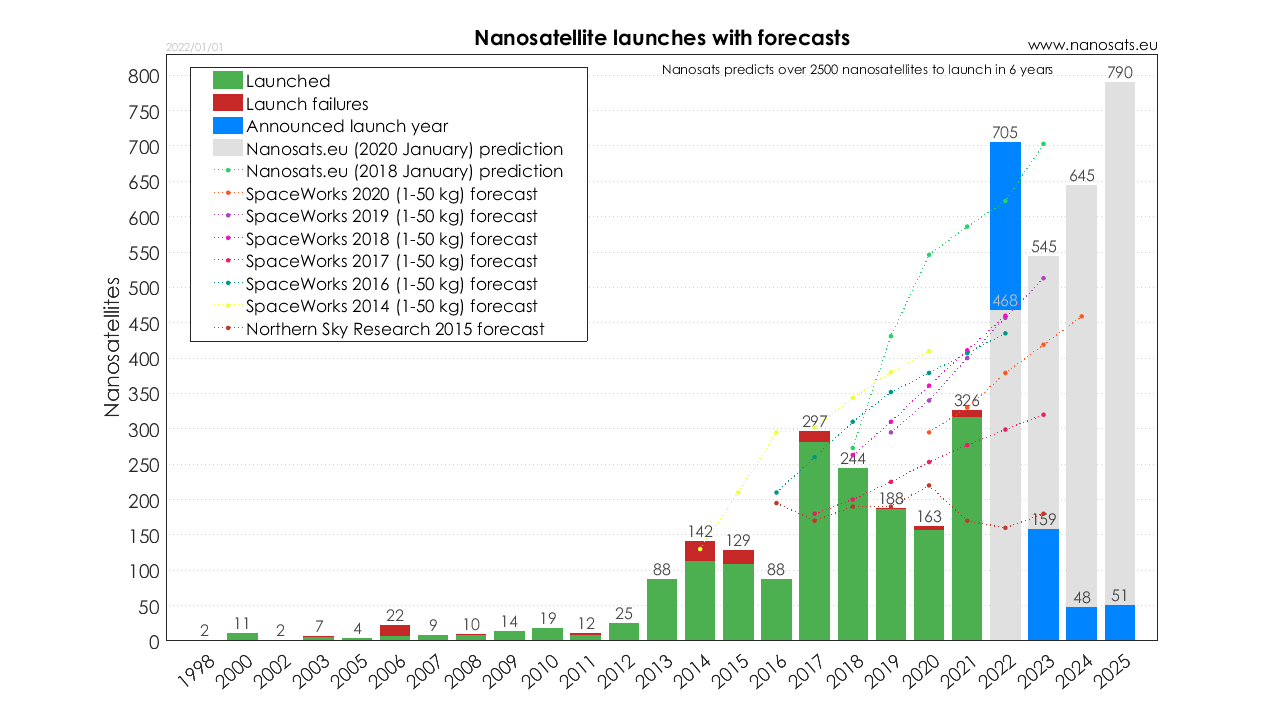
\includegraphics[width=\textwidth]{images/nanosat_years_forecast.png}
    \legend{Fonte: Nanosats Database \cite{nanosats-database}}
    \label{fig:nanosats_years_forecast}
\end{figure}


\section{Qualification and validation test methodology of the
open-source CubeSat FloripaSat-I \cite{marcelino2020-2}}

Esta seção e a próxima apresentam dois trabalhos produzidos como resultado da missão FloripaSat-1, uma missão de demonstração desenvolvida inteiramente por estudantes da Universidade Federal de Santa Catarina (UFSC), cujo CubeSat foi lançado em 2019.

O FloripaSat-1 é composto de três módulos distintos, o sistema elétrico - EPS (\textit{Electric Power System}), o módulo de gerência de dados - OBDH (\textit{Onboard Data Handling}) e o módulo de telemetria e telecomandos - TT\&C (\textit{Telemetry, Tracking and Command}).

O artigo informa que a missão tinha como objetivo testar tecnologias que possibilitem o desenvolvimento rápido e de baixo custo de satélites espaciais, além de treinar estudantes nas áreas de concepção, implementação e operação de uma missão espacial completa. Além disso, o FloripaSat-1 é um projeto \textit{open source} e as informações de software e hardware dos módulos desenvolvidos estão disponíveis em repositórios públicos, para uso em futuras missões.

Os autores descrevem que o FloripaSat-1 foi desenvolvido com base em projetos de engenharia de sistemas, dividido em Modelos de protótipo (PM), engenharia (EM-I e EM-II) e finalmente o Modelo de Vôo (FM). Foram realizados testes em cada uma dessas etapas para validar os sistemas e os resultados, segundo o artigo, foram decisivos na detecção e correção de erros.

Apesar do artigo focar em integração e validação dos módulos a nível de hardware, julga-se relevante para a elaboração deste trabalho, que foca principalmente em software, por descrever as diferentes condições que uma missão espacial é submetida, além da metodologia de desenvolvimento adotada pela equipe do FloripaSat-1, em que a grande maioria dos membros seguiu para a missão FloripaSat-2, a qual este trabalho se baseia.

\section{A Critical Embedded System Challenge: The
FloripaSat-1 Mission \cite{marcelino2020-1}}

Este artigo, elaborado também a partir da missão FloripaSat-1 do SpaceLab, apresenta definições e descrições dos subsistemas do satélite, além de algumas informações e resultados de testes e simulações realizadas nos mesmos.

Como descrito anteriormente, o FloripaSat-1 possui três sub sistemas principais:

\begin{itemize}
    \item \textit{Electric Power System} (EPS)
    \item \textit{On-Board Data Handling} (OBDH)
    \item \textit{Tracking, Telemetry and Command} (TT\&C)
\end{itemize}

O EPS é o módulo responsável por distribuir, coletar e armazenar a energia utilizada pelo satélite. A energia é coletada através de painéis solares e armazenada em uma bateria de íon de lítio. A distribuição da energia é definida a partir de um microcontrolador que analisa os estados de carga e de energia e decide quais módulos permanecerão em operação.

O OBDH é o módulo responsável pela gerência de atividades do satélite. Ele realiza a interface entre todos os subsistemas do satélite. Os dados gerados são empacotados e transmitidos através do TT\&C, e dados recebidos são enviados ao OBDH para que ele execute a tarefa requisitada, ou então envie o comando ao módulo requisitado. Este módulo também possui uma memória, para que possam ser futuramente recuperados.

Finalmente, o TT\&C é o módulo responsável pela comunicação entre o satélite e as estações de controle na Terra. Ele opera através de dois módulos de rádio, um para a banda VHF e um para UHF. Os comandos a serem enviados e recebidos pelo satélite (\textit{downlink}/ \textit{uplink}) são transmitidos através do módulo UHF e a banda VHF é reservada para transmissões do tipo \textit{beacon}.

Os autores discorrem ainda sobre os demais módulos e subsistemas do satélite, como outros \textit{payloads} que não foram desenvolvidos ou projetados pela equipe da UFSC e portanto, ficam de fora desse breve resumo.

A relevância deste artigo se dá pelo fato de que o FloripaSat-2 utiliza a mesma estrutura de subsistemas, com os seus módulos sendo sucessores diretos do software e hardware utilizados na missão anterior, operando de forma idêntica ou muito similar.


%

\section{Considerações}

Os trabalhos relacionados escolhidos têm como principal função estabeler a importância de uma estrutura de testes bem fundamentada. Todos os trabalhos mencionam que a etapa de testes foi importante pra a descoberta e solução de erros que não foram descobertos ou detectados durante os ciclos de desenvolvimento normais.

Além disso, os dois trabalhos produzidos por estudantes do SpaceLab como resultado da missão FloripaSat-1 mostram a importância de CubeSats como ferramenta educacional, servindo para treinar e capacitar estudantes no projeto, desenvolvimento e operação de uma missão espacial completa.

O modelo proposto por este trabalho é uma continuidade desse pensamento: possibilitar mais uma ferramenta de testes que possa resultar em maior confiabilidade dos sistemas embarcados desenvolvidos para o FloripaSat-2, fazendo uso do ambiente de aprendizado e da experiência adquirida durante o desenvolvimento da missão.

\iffalse

\fi